\chapter{Modélisations de l'audiovisuel (m,i)}\label{chap:mav}
%
Il existe de nombreux modèles, schémas et standards pour décrire les divers aspects de la chaîne de production et des objets qui y sont construits. 
Certains de ces standards sont issues d'une refléxion plus générale et doivent être adaptés aux besoins de l'audiovisuel. 
C'est le cas par exemple du schéma de métadonnées Terms de la \pc{Dublin Core Metadata Initiative} (\cite{DCMIUsageBoard2010}) qui vise à décrire toutes ressources sur le Web, dont une spécialisation a été proposé par \cite{Hunter1999}.
D'autres adoptent une approche générale qui englobe l'ensemble des contenus multimédia.
Le \pc{Moving Picture Experts Group} (MPEG) est certainement l'organisation qui a le plus porté cette vision avec leurs standards MPEG-7 et MPEG-21.
Enfin, il y a des modèles développés spécifiquement par des membres de l'industrie pour répondre aux besoins de l'audiovisuel ou de la télévision. 
Il s'agit par exemple d'organisation comme le \pc{TV Anytime Forum}, la \pc{Society of Motion Picture and Television Engineers} (SMPTE) et l'\pc{Union Européenne de Radio-télévision} (UER ou EBU en anglais).

Nous proposons d'examiner ces modélisations de l'audiovisuel à partir de la spécifications de nos problèmes (section \ref{sec:prob}) : 
\begin{liste}
	\item[(A)] \g{la modélisation des objets construits au fil de la chaîne de production audiovisuelle}.
	On entend ici par \gui{objets}, tous les éléments intermédiaires et finaux construits au moment de la production et de la post-production.
	Il s'agit par exemple des prises de vues, du montage que l'on en construit, des séquences qui composent le document final, des variations construites à partir de ces éléments etc. 
	On s'intéresse donc aux types d'objets audiovisuels modélisés, au niveau d'abstraction et de fragmentation proposé pour rendre compte de la composition de ces objets.\\
	% modèle de composition (\cite{Stockinger2007})

	\item[(B)] \g{la modélisation des connaissances sur ces objets}.
	Sur ce point, il s'agit de clarifier la nature des connaissances que l'on attache aux objets et leur pertinence vis-à-vis des usages que l'on prend en compte. 
	Nous considérons trois types de connaissances à associer aux objets : 
	\begin{liste}
		\item les connaissances sur les objets ; leur \e{représentation matérielle} (stockage, encodage, format etc.) ; leur \e{contenu} (ce qui est vu ou entendu par le lecteur).

		\item les connaissances liées à la chaîne de production ; la \e{spécification de la forme et du contenu} (que l'on retrouve dans les documents de pré-production) ; le \e{contexte de production} au sens large, incluant les contributeurs et leurs contributions à la chaîne ; le \e{cadre d'exploitation}  qui détaille l'usage de ces objets (type de distribution, droits et propriété intellectuelle, type de réutilisation et transformations opérées pour la réaliser, etc.).

		\item des connaissances issues de l'analyse du contenu des objets audiovisuels. 
		Par exemple, une analyse rhétorique du contenu permettra de mettre à jour la logique argumentative ou discursive (\cite{Gaillard2008}). 
		Ainsi, une multitude d'analyses peuvent être menées, chacune selon une grille d'analyse du contenu propre. 
		On examinera alors si les modélisations permettent d'ajouter de nouvelles échelles de fragmentation et d'y adjoindre des informations.
	\end{liste}
\end{liste}

% Nous présenterons d'abord un scénario de réutilisation pour clarifier les usages que nous visons ainsi que les besoins en modélisation (\ref{sec:cdc-av}).
% Notre état de l'art sera nourri par un examen préalable des définitions de l'objet audiovisuel  (section \ref{sec:dav}).


% On peut tenter de distinguer entre différents approches et objets de modélisation : 
% \begin{liste}
% 	\item \e{les modélisations de l'objet audiovisuel} : celles qui traitent de la composition d'un objet audiovisuel fini, qui détaillent la manière de représenter sa structure interne, ou bien la manière dont on l'a groupé avec d'autres objets.
% 	\item 
% \end{liste}
 

% Certains se concentrent sur la description des caractéristiques du signal, des évènements que montrent le contenu ou encore de la manière dont ces contenus sont produits, échangés, adaptés etc.

% L'objectif de ce chapitre est d'examiner les modèles de l'audiovisuel existants en regard de nos  de réutilisation des objets audiovisuels. 
% modéliser les objets de la chaîne de production et les connaissances associées

% les objets de la chaîne de production
% les connaissances associées à ces objets permettant de les rendre autonome dans leur circulation et leur réutilisation.

% Plusieurs sous-problèmes pour réaliser l'autonomie des objets audiovisuels :  
% nous examinerons la manière dont on peut définir un objet, un document, un contenu audiovisuel. 
% comment modéliser ces objets pour gérer leur circulation 
% comment modéliser ces objets pour faciliter leur réutilisation


% d'un exemple de réutilisation d'objets audiovisuels (\ref{sec:cdc-av}). 
% À 
% , qu'il s'agisse de clarifier les notions d'objet ou de document audiovisuel puis d'investir les problèmes de leur gestion et de leur description. 
% Nous poserons d'abord un exemple de réutilisation d'objet audiovisuels comme élément de base de notre réflexion (\ref{sec:ex-reuse}).

% \e{
% Qu'est-ce qu'un objet audiovisuel et particulier comment peut-on aborder le document audiovisuel ? (\ref{sec:dav})
% Comment les produits de la chaîne audiovisuelle sont gérées par les systèmes informatiques, quelles opérations sont menées sur ces objets ? (\ref{sec:gest})
% Comment décrit-on les objets audiovisuels, comment s'organisent la construction ou la récolte de ces informations dans la chaîne de production ? (\ref{sec:desc})}

\section{Cahier des charges fonctionnel}\label{sec:cdc-av}
% \addcontentsline{toc}{section}{Cahier des charges fonctionnel}



\subsection{Scénario de réutilisation multiple}\label{sec:ex-reuse}
Pour bien saisir la finesse des différentes opérations possibles, nous proposons de prendre un exemple.
Imaginons une chaîne de télévision qui souhaite réaliser la captation d'un évènement culturel (par exemple un opéra, une pièce de théâtre, un concert etc.). 
Les producteurs de la chaîne sont intéressés par trois types de contenus qui seront ensuite exploités de quatre manières différentes (voir Figure \ref{img:intro:reuse}):
\begin{listenum}
	\item[a.] la \e{captation de l'évènement} en tant que tel.
	\item[b.] des \e{entrevues avec l'équipe} (metteur en scène, talents sur scène, programmateur etc.). 
	\item[c.] des \e{commentaires du public} avant ou après l'évènement.\\

	\item une partie de tous les types de contenu sera utilisée pour construire un sujet destiné à un \e{journal télévisé}. 
	\item un montage raccourci de l'évènement et des commentaires du public seront utilisés pour produire une \e{bande-annonce diffusée sur le Web}.
	\item un montage de la captation de l'évènement, des bonus comprenant les entrevues avec l'équipe ainsi que la bande-annonce utilisant les commentaires spectateurs seront intégrés dans le \e{DVD}.	 
	\item tout ou partie du contenu filmé pourra être transmis ou vendu à des \e{organisations tierces}. 
\end{listenum}

\begin{figure}[ht!]
\centering
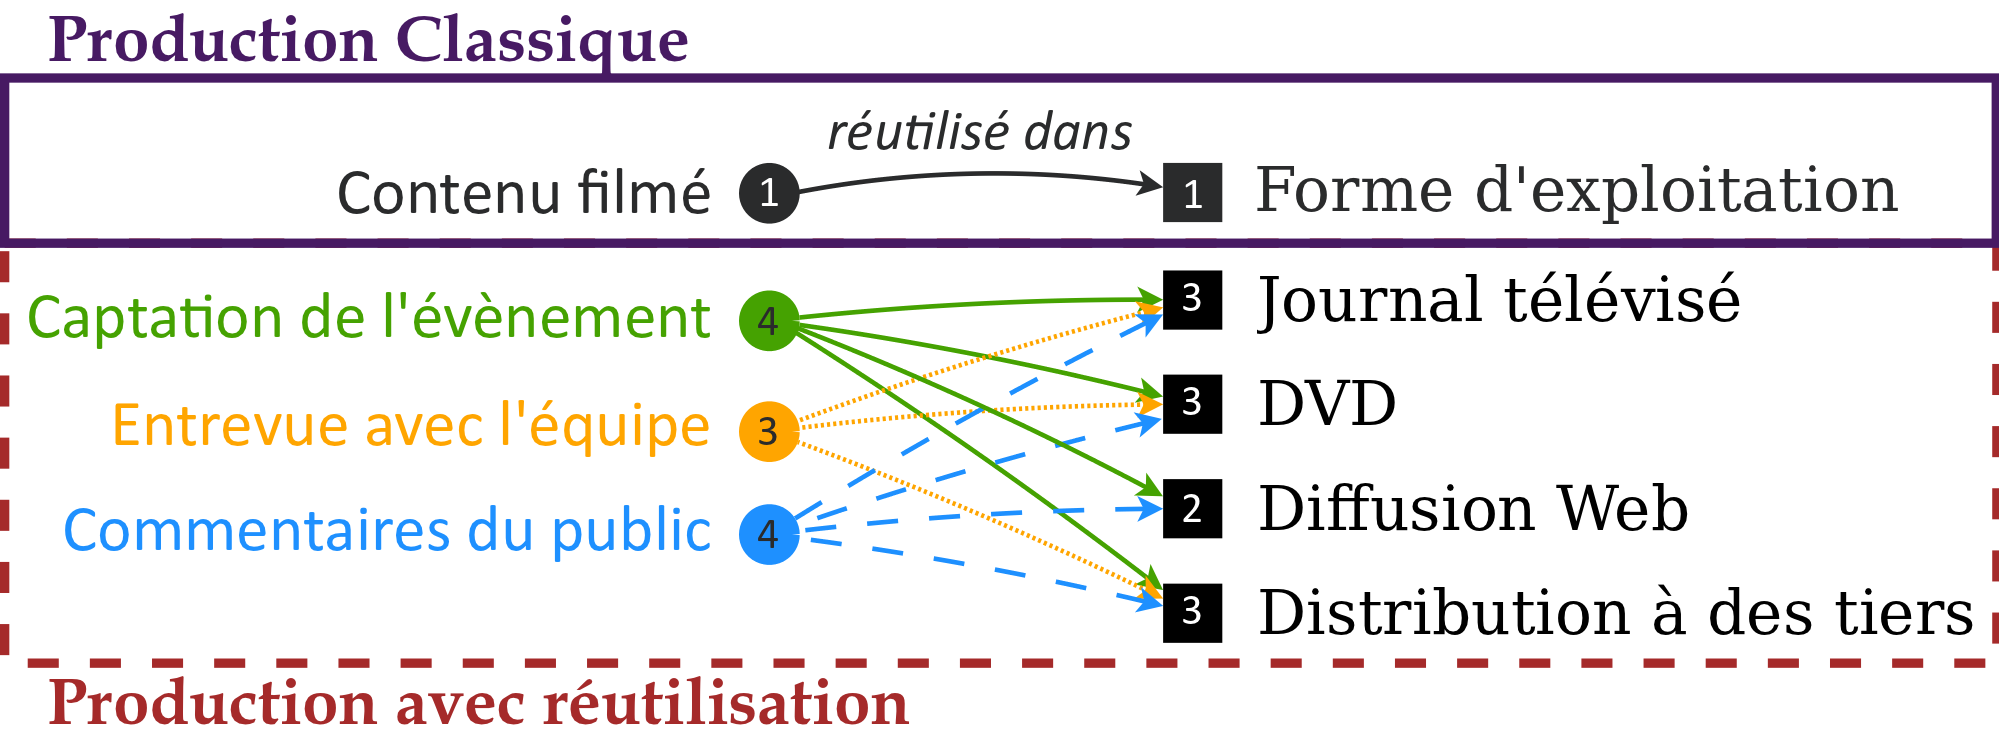
\includegraphics[width=0.7\textwidth]{images/UC-Tahnhauser-v1fr.png}
\caption{Modèle de la production classique comparé avec une production avec réutilisation}
\label{img:intro:reuse}
\end{figure}

Chaque cas de réutilisation tire sa matière première d'à peu près la même base de contenu filmé, mais en tire partie d'une manière propre à chaque forme d'exploitation visée. 
En effet, chaque audience a ses attentes, de même qu'il existe des contraintes techniques spécifiques pour chaque contexte d'exploitation. 
%En effet, il existe des contraintes techniques et des attentes spécifiques à chaque contexte d'exploitation. 

Ces spécificités exigent des variations dans la qualité de l'encodage, le format d'encapsulation utilisé, le montage réalisé, l'habillage du contenu etc. 
Par exemple, les contraintes de diffusion sur le Web implique d'encoder la vidéo dans un format spécifique et de multiples résolutions, généralement plus petites que pour la diffusion télévisée. 
Ensuite, le montage d'une bande-annonce possède un rythme généralement plus rapide que celui des bonus de DVD. 
Finalement, les cas d'exploitation gérés par la chaîne de télévision posséderont un habillage spécifique (logo de la chaîne, message d'annonces etc.) que ne partageront pas forcément les versions vendu à des organisations tierces. 

L'exemple des commentaires du public -- voir la Figure \ref{img:intro:reuse-process} -- permet de montrer à quels moments des transformations doivent être effectuées afin de produire les différentes formes d'exploitation :
\begin{liste} 
	\item[$\bullet$] On considère que deux commentaires de spectateur ont été tournés. 
	\item[$\bullet$] Un des commentaires est intégré au montage du journal télévisé, alors que les deux sont utilisés pour créer la bande-annonce. La bande-annonce est elle-même intégrée au montage du DVD. 
	\item[$\bullet$] Au moment de la finition, l'encodage de la bande-annonce est adapté à la qualité DVD et Web. De même, le journal télévisé est encodé à la fois pour une diffusion en définition standard (SD) et haute-définition (HD).
\end{liste}


\begin{figure}[ht!]
\centering
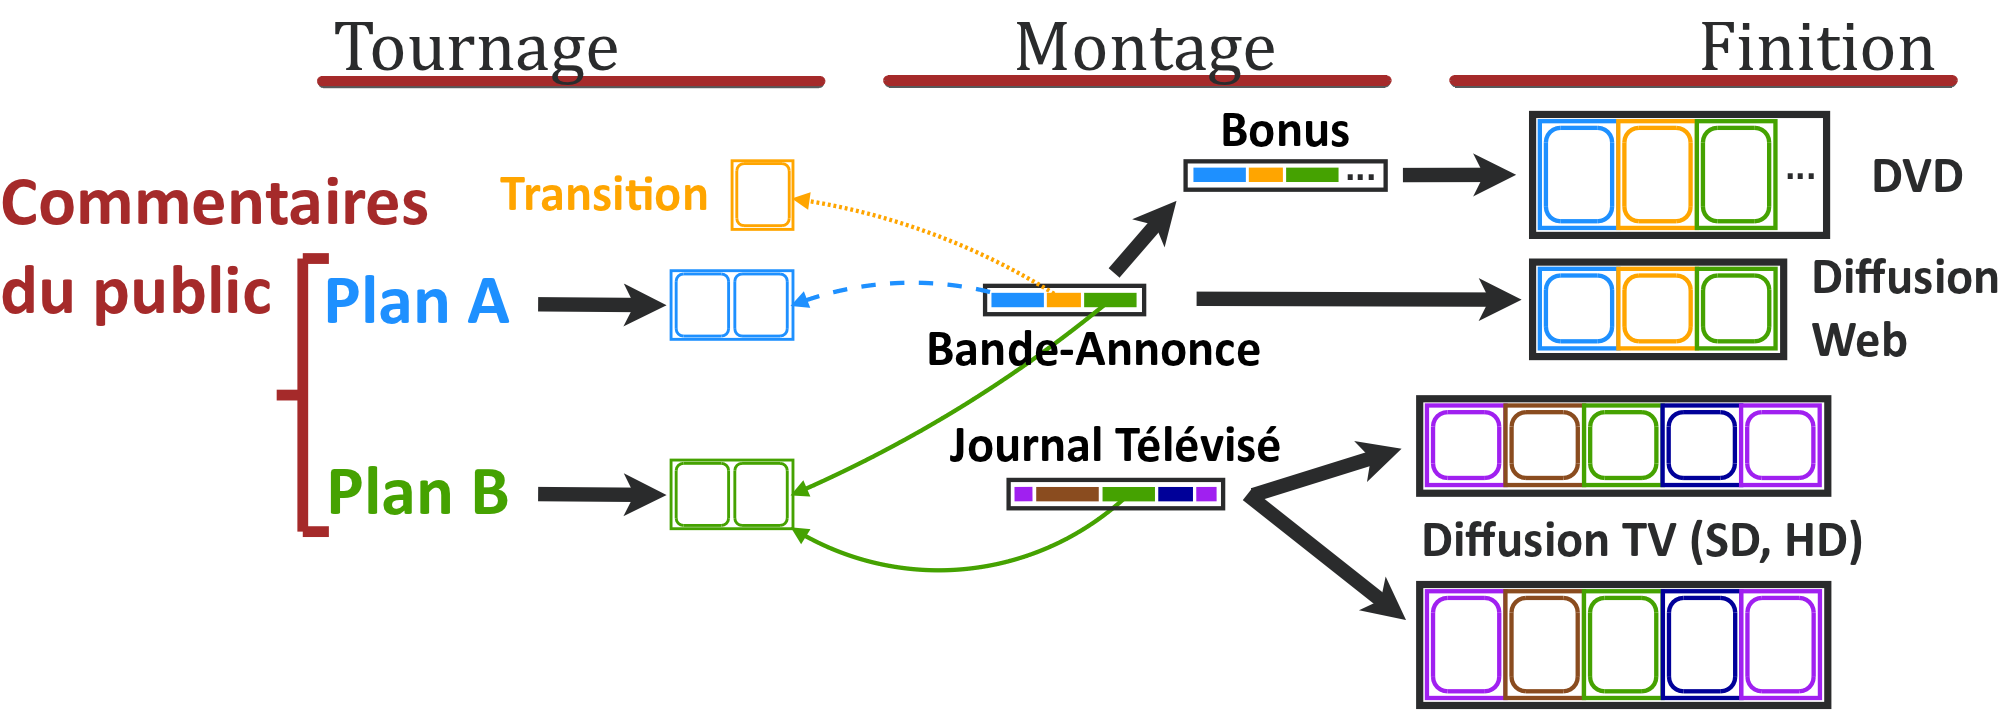
\includegraphics[width=0.8\textwidth]{images/EX-Content-Production-v7fr.png}
\caption{Étapes et transformations des contenus pour chaque forme d'exploitation des commentaires des spectateurs}
\label{img:intro:reuse-process}
\end{figure}

% Dans cet exemple, on distingue deux types d'opérations effectuées sur le contenu ; 
% la sélection de séquences au moment du montage qui correspond à une décision éditoriale (quel contenu va-t-on présenter à l'audience ?) ; 
% la tranformation de l'enregistrement du contenu qui correspond à des choix techniques (quelle méthode d'enregistrement va-t-on utiliser ?).
% Afin de préciser la nature de ces opérations, nous présentons différentes approches de la réutilisation des contenus.


\subsection{Besoins en modélisation (n,i,t)}
The details of this use case specifies more than a simple reuse of material. It specifies the kind of processing that support repurposing and which defines thus the modeling requirements for the audiovisual document:
%Such exploitation cases implies various kinds of operations: 
\begin{itemize}
	\item the \textit{reencoding} of edited material to fit the technical parameters proper to each distribution medium/channel (news report distributed by channel broadcasting and internet).
	
	\item the reuse of shooting materials in two distinct editorial structure (\textit{resequencing} of the opinion shot in the website and news report editing).

	\item the reuse of a part of an editorial structure into another editorial structure (\textit{repurposing} of the public comment editing into the DVD bonus editing). 
\end{itemize}

